\section{Introduction}

% --------------------------------------------------------------------------------------------------------------
\begin{frame}
\frametitle{Pagerank}
\begin{figure}
	\centering
	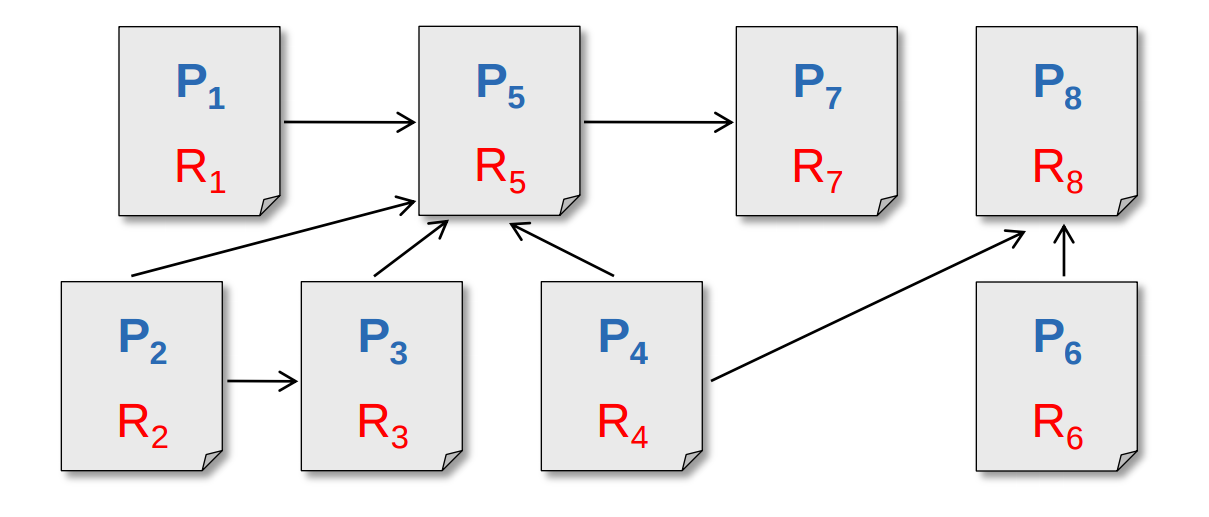
\includegraphics[width=0.8\textwidth]{pagerank1.png}
	\caption{PageRank example 1 \cite{prsigner}}
\end{figure}
\begin{itemize}
  \item A page has a high PageRank $R$ if
  \begin{itemize}
    \item there are many pages linking to it
    \item or, if there are some pages with a high PageRank
linking to it
  \end{itemize}
\end{itemize}
\end{frame}
% --------------------------------------------------------------------------------------------------------------

% --------------------------------------------------------------------------------------------------------------
\begin{frame}
\frametitle{Pagerank}

\begin{minipage}[l]{0.5\textwidth}
\textbf{$$ 
R(P_i)= \sum_{P_j \in B_i}\frac{R(P_j)}{L_j}
$$}
\begin{itemize}
  \item where
  \begin{itemize}
    \item $B_i$ is the set of pages that link to page $P_i$
    \item $L_j$ is the number of outgoing links for page $P_j$
linking to it
  \end{itemize}
\end{itemize}
\end{minipage}
\begin{minipage}[l]{0.49\textwidth}
\begin{figure}
	\centering
	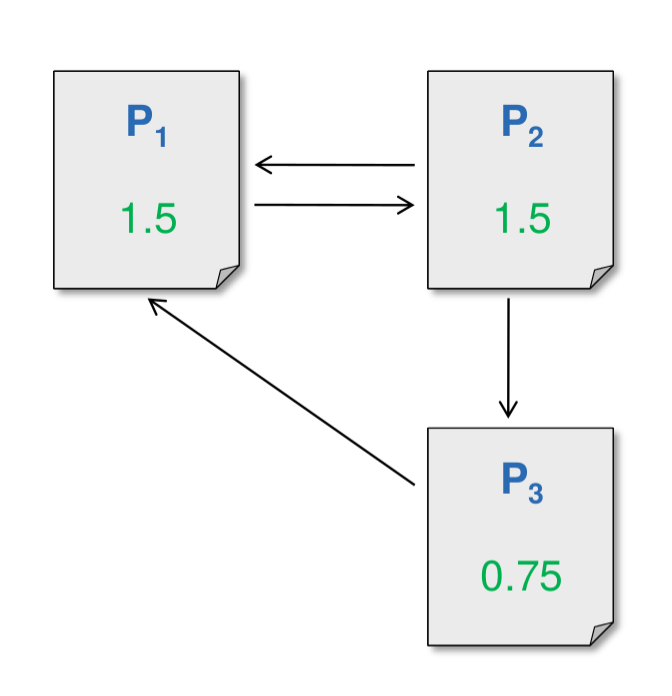
\includegraphics[width=\textwidth]{pagerank2.png}
	\caption{PageRank example 2 \cite{prsigner}}
\end{figure}
\end{minipage}

\end{frame}
% --------------------------------------------------------------------------------------------------------------

% --------------------------------------------------------------------------------------------------------------
\begin{frame}
\begin{figure}
	\centering
	
\includegraphics[width=0.65\textwidth]{squirrel.png}
	\caption*{\cite{squirrel}}
\end{figure}
\end{frame}
% --------------------------------------------------------------------------------------------------------------

% --------------------------------------------------------------------------------------------------------------
\begin{frame}
\frametitle{Apache Flink}
\begin{itemize}
\item Open source framework for distributed Big Data Analytics
\item Exploits:
	\begin{itemize}
	\item data streaming
	\item in-memory processing
	\item iteration operators
	\end{itemize}
to improve performance
\item Formerly Stratosphere (Flink means agile)
\item Developped here at TUB
\end{itemize}
\end{frame}
% --------------------------------------------------------------------------------------------------------------

% --------------------------------------------------------------------------------------------------------------
\begin{frame}
\begin{figure}
	\centering
	
\includegraphics[width=0.9\textwidth]{repetition.jpg}
	\caption*{\cite{repetition}}
\end{figure}
\end{frame}
% --------------------------------------------------------------------------------------------------------------

% --------------------------------------------------------------------------------------------------------------
\begin{frame}
\frametitle{Apache Flink: 2 possible setups}

\begin{minipage}[l]{0.5\textwidth}
\begin{figure}
	\centering
	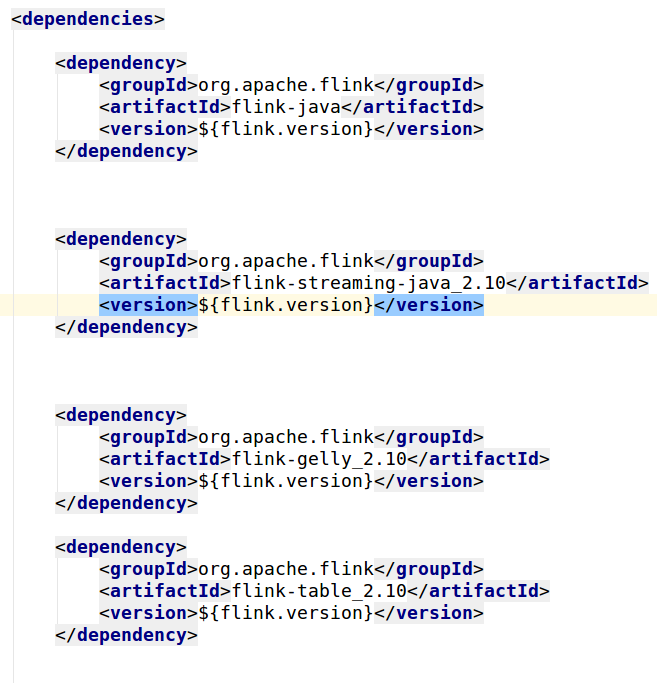
\includegraphics[width=0.9\textwidth]{pomxml.png}
	\caption{Maven}
\end{figure}
\end{minipage}
\begin{minipage}[l]{0.49\textwidth}
\begin{figure}
	\centering
	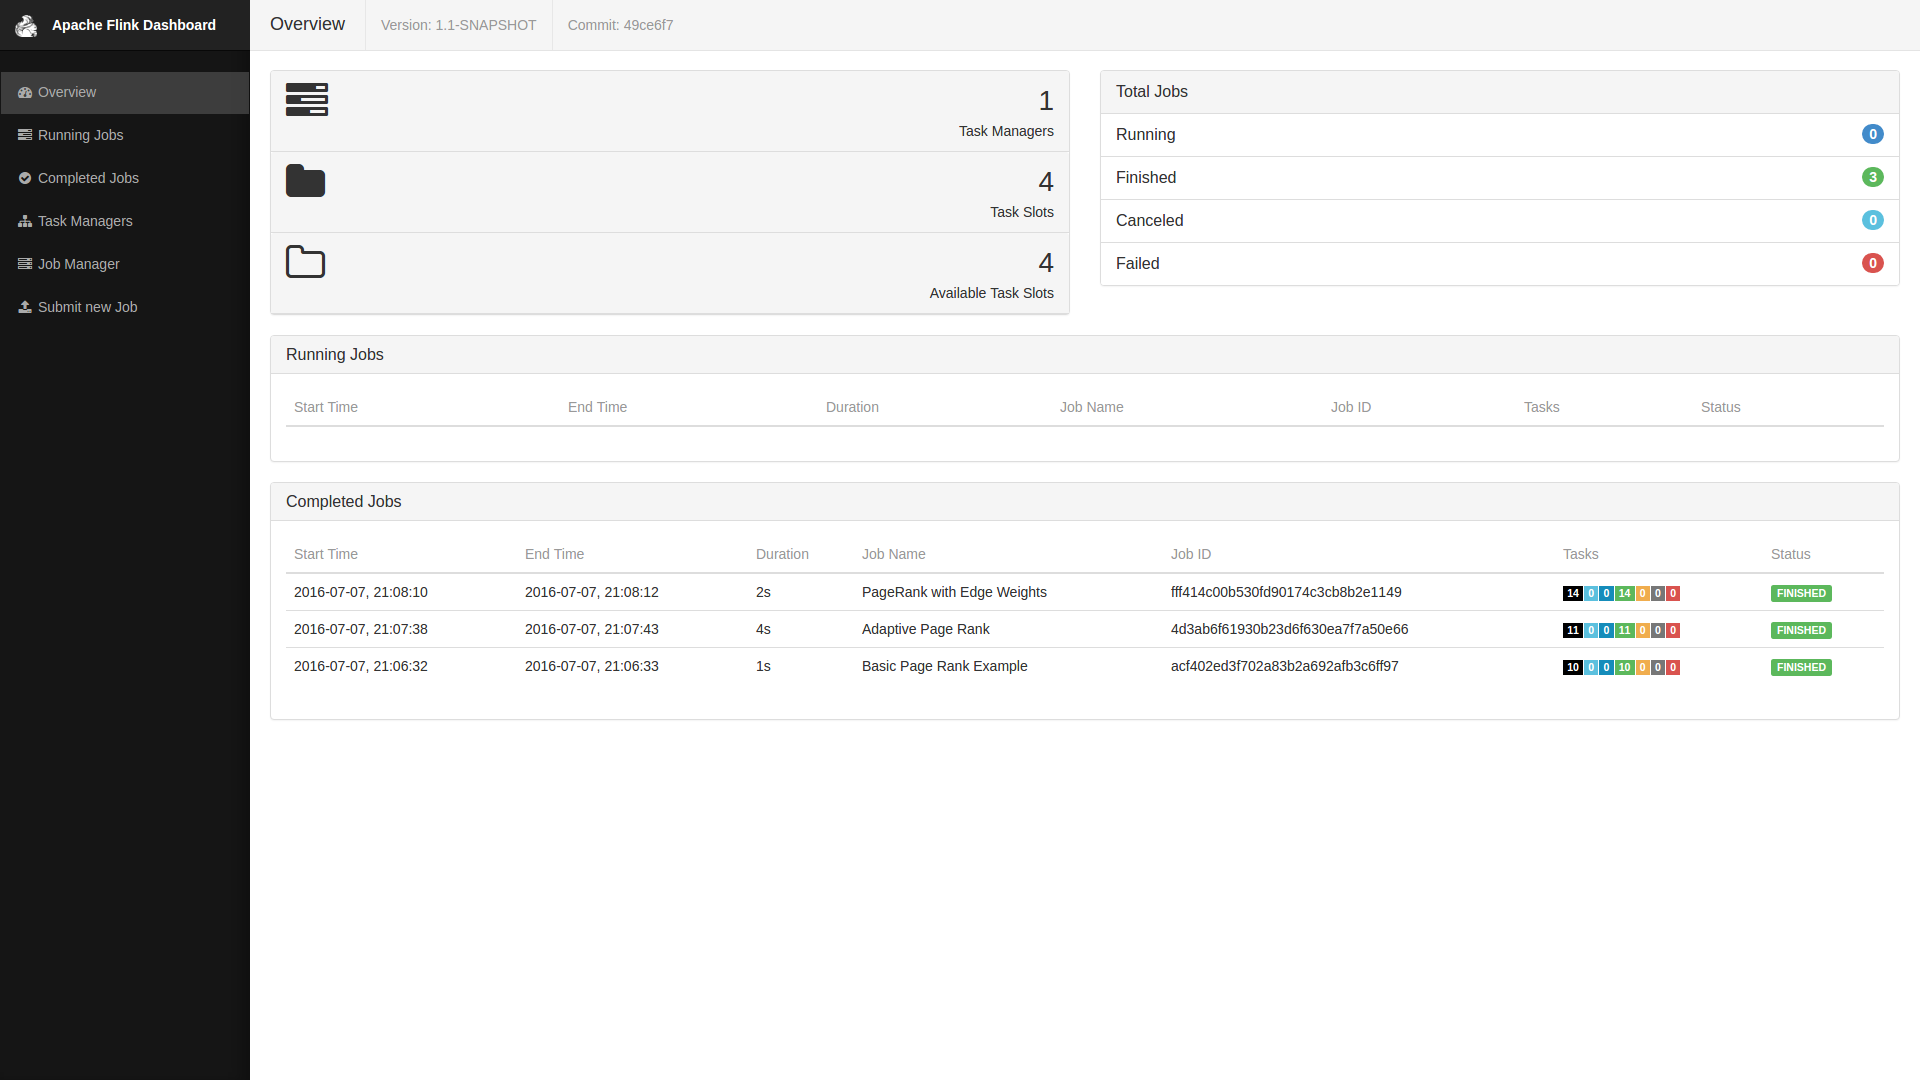
\includegraphics[width=\textwidth]{dashboard.png}
	\caption{Binary version (self compiled)}
\end{figure}
\end{minipage}
\end{frame}
% --------------------------------------------------------------------------------------------------------------

% --------------------------------------------------------------------------------------------------------------
\begin{frame}
\frametitle{Apache Flink: Gelly}

\begin{figure}
	\centering
	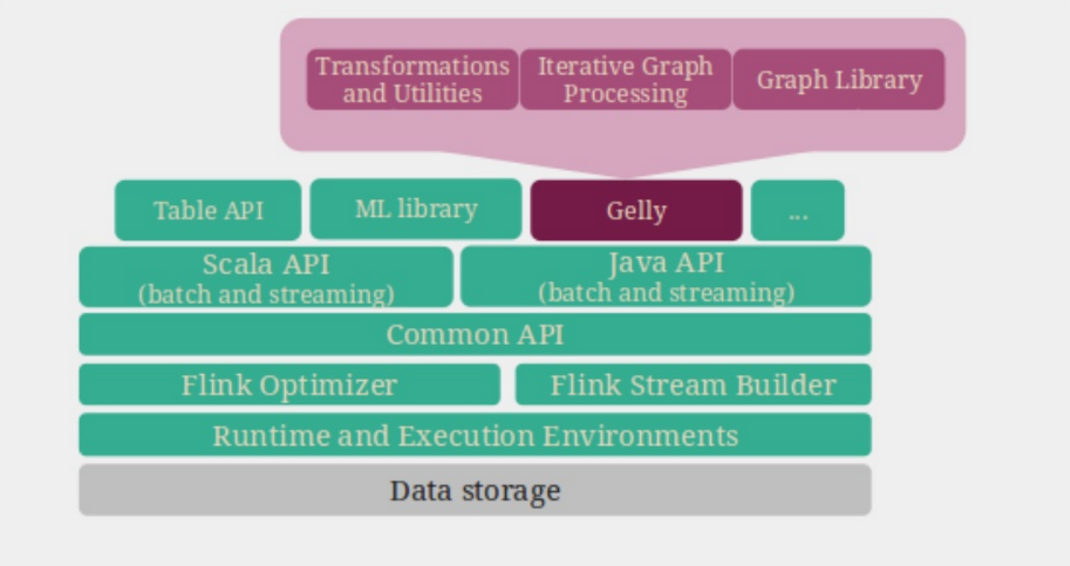
\includegraphics[width=\textwidth]{gelly.png}
	\caption{Gelly}
\end{figure}

\end{frame}
% --------------------------------------------------------------------------------------------------------------

% --------------------------------------------------------------------------------------------------------------
\begin{frame}
\frametitle{Apache Flink: Gelly}
\begin{itemize}
\item Large-scale graph processing API
\item On top of Flink's Java API
\item Off-the shelf library methods (e.g. pagerank)
\item Iterative algorithms
\end{itemize}


\end{frame}
% --------------------------------------------------------------------------------------------------------------
